\documentclass[12pt, twoside]{article}

% Bibliography.
\usepackage{cite}

\newcommand{\reporttitle}{The \textit{hp-Adaptive} Discontinuous Galërkin Method}
\newcommand{\accentcolor}{solarized-blue}
\newcommand{\urlcolor}{\accentcolor}

\usepackage{amsmath}
\usepackage{mathrsfs}
\usepackage{amsthm}
\usepackage{amsfonts}
\usepackage{bm}
\usepackage{amssymb}
\usepackage{stmaryrd}

% Sets and spaces.
\newcommand{\R}{\mathbb{R}}
\newcommand{\RT}{\mathbb{R}^2}
\newcommand{\N}{\mathbb{N}}

\newcommand{\PK}[1]{\mathbb{P}_{#1}}

\newcommand{\LT}{\mathscr{L}^2}
\newcommand{\HO}{\mathscr{H}^1}

\newcommand{\Tau}{\mathcal{T}}
\newcommand{\F}{\mathcal{F}}

% Vectors and operators.
\newcommand{\Vector}[1]{\bm{#1}}
\newcommand{\Operator}[1]{\textcolor{solarized-cyan}{#1}}

% Matrices.
\newcommand{\MM}{\mathcal{M}}
\newcommand{\MA}{\mathcal{A}}
\newcommand{\VB}{\mathcal{B}}

% Gradient and divergence.
\newcommand{\grad}{\Vector{\nabla}}
\newcommand{\diver}{\text{div }}

% Span.
\newcommand{\Span}[1]{\text{span} \left\{ #1 \right\}}

% Bilinear operators.
\newcommand{\boa}[2]{\Operator{a}(#1, #2)}

% Redefinition.
\newcommand{\Exists}{\exists ~}
\newcommand{\Forall}{\forall ~}

% Theorems.
\newtheorem{theorem}{Theorem}[section]
\newtheorem{lemma}{Lemma}[section]
\newtheorem{proposition}{Proposition}[section]

\newtheorem*{theorem*}{Theorem}

\usepackage{courier}
\usepackage{listings}

\lstdefinestyle{default}{
	basicstyle=\ttfamily\color{solarized-base01},
	breakatwhitespace=false,
	breaklines=true,
	keepspaces=true,
	showspaces=false,
	showstringspaces=false,
	showtabs=false,
	tabsize=2
}

\lstdefinestyle{cpp}{ % C++
	commentstyle=\color{solarized-green},
	keywordstyle=\color{solarized-blue},
	stringstyle=\color{solarized-orange},
	basicstyle=\ttfamily\color{solarized-base02},
	numberstyle=\ttfamily\color{solarized-base01},
	breakatwhitespace=false,
	breaklines=true,
	captionpos=b,
	keepspaces=true,
	showspaces=false,
	language=c++,
	showstringspaces=false,
	showtabs=false,
	numbers=left,
	tabsize=4
}

\lstset{style=default}

\usepackage{nameref}
\usepackage{multicol}
\usepackage{titlesec}

\usepackage{enumerate}

\usepackage{graphicx}
\graphicspath{{gallery/}}

% Plots.
\usepackage{subcaption}

% TikZ.
\usepackage{tikz}
\usepackage{pgfplots}
\pgfplotsset{compat=1.18}

\usepackage{xcolor-solarized}
\color{solarized-base02}

\usepackage[T1]{fontenc}
\usepackage[utf8]{inputenc}

\usepackage[a4paper]{geometry}
\geometry{
	inner=20mm,
	outer=20mm,
	top=30mm,
	bottom=30mm,
	heightrounded,
	marginparwidth=50pt,
	marginparsep=20pt,
	headsep=25pt,
	headheight=30pt
}

% Paragraph spacing.
\usepackage{parskip}

\usepackage{hyperref}
\hypersetup{
	linktocpage=true,
	colorlinks=true,
	linkcolor=\accentcolor,
	urlcolor=\urlcolor,
	citecolor=\accentcolor,
	pdftitle={\reporttitle},
	pdfpagemode=FullScreen,
	pdfauthor={Andrea Di Antonio}
}

\usepackage{fancyhdr}
\pagestyle{fancy}
\fancyhf{}
\fancyhead[R]{Andrea Di Antonio}
\fancyhead[EL]{\reporttitle}
\fancyhead[OL]{Advanced Programming for Scientific Computing}
\fancyfoot[C]{\thepage}

\title{\reporttitle}
\author{Andrea Di Antonio\footnote{UniMiB: 858798, PoliMi: 10655477.} \\ Supervised by Professors Paola F. Antonietti and Marco Verani} % Add supervisors.
\date{Exam session of September 10th, 2024 \\ Academic Year 2023-24}

\setcounter{tocdepth}{3}

\begin{document}
	\pagenumbering{roman}
	\maketitle
	\thispagestyle{fancy}

	\begin{abstract}
		\begin{center}
			This report details the implementation of the \textit{hp-adaptive} discontinuous Galërkin method, as part of the course \textit{Advanced Programming for Scientific Computing}. It covers key aspects including mesh generation, problem solving, and the integration of \textit{hp-adaptivity}. For technical details, refer to the project repository on \href{https://github.com/diantonioandrea/pacs-project}{GitHub}.
		\end{center}
	\end{abstract}

	\newpage
	\tableofcontents

	\newpage
	\pagenumbering{arabic}
    \section{Introduction}
	Consider the domain $\Omega \subset \mathbb{R}^2$. The aim is to find $u \in C^2(\Omega)$ such that, for any $f \in C(\Omega)$, the following hold:

\begin{gather}
    \begin{cases} \label{strong_stokes}
        - \Delta u = f & \Forall \Vector{x} \in \Omega, \\
        u = 0 & \Forall \Vector{x} \in \partial \Omega.
    \end{cases}
\end{gather}

\subsection{Weak formulation}

Now, seeking $u \in \HO_0(\Omega) = V$ such that, given $f \in V^*$, the following equation is satisfied:

\begin{gather} \label{weak_stokes}
    \boa{u}{v} = \langle f, v \rangle \quad \Forall v \in V,
\end{gather}

where $\boa{\cdot}{\cdot}: V \times V \rightarrow \mathbb{R}$ is defined as follows:

\begin{gather}
    \boa{u}{v} = \int_{\Omega} \grad u \cdot \grad v ~ d \omega. \label{a}
\end{gather}

	\newpage
    \section{Polygonal Meshes Over a Polygonal Domain}
	\subsection{Building a mesh}

\begin{frame}
    \frametitle{Mesh-Building Strategy}

    The mesh-building strategy follows these steps:

    \begin{enumerate}
        \item Voronoi diagram generation,
        \item Diagram relaxation,
        \item Small edge collapse,
        \item Element connectivity analysis,
        \item Property evaluation.
    \end{enumerate}

    This process is facilitated by a thorough implementation of analytic geometry operations, including those involving lines and polygons.
\end{frame}

\begin{frame}[fragile]
    \frametitle{\lstinline{mesh_diagram}, \lstinline{mesh_relax}}

    Most steps of the mesh-building process are carried out by \lstinline{mesh_diagram}\footnote{Building and postprocessing.} and \lstinline{mesh_relax}.

    \begin{lstlisting}[style=cpp]
    std::vector<Polygon> mesh_diagram(
        const Polygon &, 
        const std::size_t &, 
        const bool &reflect = false, 
        const bool &uniform = false);

    std::vector<Polygon> mesh_relax(
        const Polygon &, 
        const std::vector<Polygon> &, 
        const bool &reflect = false);
    \end{lstlisting}

\end{frame}

\begin{frame}[fragile]
    \frametitle{\lstinline{Mesh}}

    \lstinline{Mesh} requires a polygonal domain, a diagram, and information on the elements' degrees.

    \begin{lstlisting}[style=cpp]
    Mesh(
        const Polygon &, 
        const std::vector<Polygon> &, 
        const std::vector<std::size_t> &);

    Mesh(
        const Polygon &, 
        const std::vector<Polygon> &, 
        const std::size_t &degree = 1);

    Element(
        const Polygon &, 
        const std::size_t &);
    \end{lstlisting}

\end{frame}

\begin{frame}[fragile]
    \frametitle{\lstinline{Mesh} methods}

    The following methods are invoked by the mesh constructors to evaluate the diagram's properties.

    \begin{lstlisting}[style=cpp]
    std::vector<Element> mesh_elements(
        const std::vector<Polygon> &, 
        const std::vector<std::size_t> &);

    std::vector<std::vector<std::array<int, 3>>> 
        mesh_neighbours(
            const Polygon &, 
            const std::vector<Element> &);

    std::vector<Real> mesh_areas(
        const std::vector<Polygon> &);

    std::vector<Vector<Real>> mesh_max_simplices(
        const std::vector<Polygon> &);
    \end{lstlisting}

\end{frame}

\subsection{Examples}

\begin{frame}[fragile]
    \frametitle{A code snippet}

    The steps to create a mesh are schematized as follows:

    \begin{lstlisting}[style=cpp]
    Point a{0.0, 0.0};
    Point b{1.0, 0.0};
    Point c{1.0, 1.0};
    Point d{0.0, 1.0};

    Polygon domain{{a, b, c, d}};

    std::vector<Polygon> diagram = 
        mesh_diagram(domain, 100);
    
    Mesh mesh{domain, diagram};
    \end{lstlisting}

\end{frame}

\begin{frame}[fragile]
    \frametitle{A repository snippet}

    Building a mesh over a square or L-shaped domain is as simple as calling one of the two scripts provided with the repository.

    To create a mesh over a square domain with $N = 250$, simply compile the domain scripts by:

    \begin{lstlisting}
    make domains
    \end{lstlisting}

    and then use the \lstinline{square_domain} script by:

    \begin{lstlisting}
    ./executables/square_domain.out 250
    \end{lstlisting}

    Use \lstinline{polyplot} to show the newly created mesh:

    \begin{lstlisting}
    ./scripts/polyplot.py output/square_250.poly
    \end{lstlisting}

\end{frame}

	\newpage
    \section{Solving the Poisson Problem}
	Having built a mesh over a polygonal domain, the Poisson problem can be solved by first constructing the problem's matrix $\MA$ and the forcing term $\VB$ as described in \eqref{matrix} and \eqref{forcing}.

The \lstinline{laplacian} function constructs the matrices used for solving the problem and evaluating errors by computing all terms in \eqref{boa} for each element. The resulting matrices are in sparse form.

The \lstinline{forcing} function constructs the forcing term by evaluating \eqref{forcing} and enforces the Dirichlet boundary condition \eqref{dirichlet} through penalization.

\cite{Saad2003} The solution to the matrix equation $\MA \Vector{\upsilon}^k_h = \VB$ is obtained using the \lstinline{BICGSTAB} algorithm, with the \lstinline{GMRES} algorithm used if the first one fails to converge within a fixed number of steps. Both of these iterative algorithms for sparse matrices have been implemented in the \textit{algebra} section of the code.

On adaptively refined meshes, $\kappa(\MA)$ rapidly grows, necessitating the use of a preconditioner within the custom solver \lstinline{lapsolver}.

Let $\MM$ and $\MA_{DG}$ be the mass and $DG$ matrices. The $L^2$ and $DG$ errors are then evaluated by first computing the modal coefficients $\Vector{\upsilon}_m$ for the exact solution $u$ and solving $\MM \Vector{u} = \Vector{\upsilon}_m$ using the \lstinline{DB}\footnote{Block diagonal algorithm.} algorithm. Thus, the error vector is $\Vector{e} = \Vector{\upsilon} - \Vector{\upsilon}^k_h$. Hence:

\begin{gather}
    \lVert u - u^k_h \rVert_{\LT(\Omega)} = \sqrt{\Vector{e}^\intercal \MM \Vector{e}}, \\
    \lVert u - u^k_h \rVert_{DG} = \sqrt{\Vector{e}^\intercal \MA_{DG} \Vector{e}}.
\end{gather}

Some examples are provided in the following sections.

\newpage
\subsection{A code snippet}

Here's a snippet to illustrate the Poisson solution process from the user's perspective:

\lstinputlisting[style=cpp, firstline=11]{../snippets/poisson.cpp}

	\newpage
    \section{Tests over a Sequence of Uniform Meshes}
	\subsection{Smooth solutions}

Tests over a sequence of uniform meshes have been conducted to verify the algorithm's performance, confirming that:

\begin{gather} \label{trends}
    \lVert u - u^k_h \rVert_{\LT(\Omega)} \approx h^{k + 1}, \\
    \lVert u - u^k_h \rVert_{DG} \approx h^k.
\end{gather}

These results were obtained by selecting a smooth function as exact solution such as the following:

\begin{gather}
    u(x, y) = \sin(2 \pi x) \cos(2 \pi y),
\end{gather}

which leads to:

\begin{gather}
    f(x, y) = -\Delta u(x, y) = 8 \pi^2 \sin(2 \pi x) \cos(2 \pi y),
\end{gather}

and non-homogeneous Dirichlet boundary conditions given by the exact solution itself.

\newpage
\subsubsection{Errors}

The following shows the error trends for the $\LT$ and $DG$ errors over sequences of uniform meshes over the square and L-shaped domains. The relations presented in \eqref{trends} have been confirmed.

\begin{figure}[!ht]
	\centering
	\includegraphics[trim=0cm 0.5cm 0cm 2cm, clip, width=16cm]{square_uniform.pdf}
    \includegraphics[trim=0cm 0.5cm 0cm 2cm, clip, width=16cm]{lshape_uniform.pdf}
	\caption{$\LT$ and DG errors versus mesh size on a sequence of uniform meshes over a square domain (top) and an L-shaped domain (bottom), $k = 2$ and $N \in \{100, 200, 400, 800\}$.}
\end{figure}

\newpage
\subsubsection{Solutions}

The following shows a scatter plot of the numerical solution $u^k_h$, the exact solution $u$, and the error $|u - u^k_h|$ over the quadrature nodes.

\begin{figure}[!ht]
	\centering
	\includegraphics[trim=0cm 2.5cm 0cm 5cm, clip, width=16cm]{square_200_sol.pdf}
    \includegraphics[trim=0cm 2.5cm 0cm 5cm, clip, width=16cm]{lshape_200_sol.pdf}
	\caption{Solution plot over a square domain (top) and an L-shaped domain (bottom), $N = 200$ and $k = 2$.}
\end{figure}

\newpage
\subsection{Pathological solutions}

Tests over a sequence of uniform meshes, using pathological functions as exact solutions, highlight the need for an adaptive algorithm.

\cite{Antonietti2013} The pathological function for the square domain is:

\begin{gather}
    u(x, y) = \frac{1 - e^{-100x}}{1 - e^{-100}} \sin(\pi y) (1 - x),
\end{gather}

which exhibits a strong boundary layer along the line $x = 0$.

For the L-shaped domain, the pathological function is:

\begin{gather}
    u(\rho, \theta) = \rho^{2 / 3} \sin\left(\frac{2 \theta}{3}\right),
\end{gather}

for which we have $f = 0$ and we know that $u$ is analytical in $\Omega \setminus \Vector{0}$, but $\grad{u}$ is singular at the origin.

\newpage
\subsubsection{Errors}

\begin{figure}[!ht]
	\centering
	\includegraphics[trim=0cm 0.5cm 0cm 2cm, clip, width=16cm]{square_uniform_pat.pdf}
    \includegraphics[trim=0cm 0.5cm 0cm 2cm, clip, width=16cm]{lshape_uniform_pat.pdf}
	\caption{$\LT$ and DG errors versus mesh size on a sequence of uniform meshes over a square domain (top) and an L-shaped domain (bottom), $k = 2$ and $N \in \{100, 200, 400, 800\}$.}
\end{figure}

\newpage
\subsubsection{Solutions}

The following plot shows that the error in these particular solutions is strongly localized, indicating that uniform refinement cannot perform optimally, also considering its rapidly growing computational cost.

\begin{figure}[!ht]
	\centering
	\includegraphics[trim=0cm 2.5cm 0cm 5cm, clip, width=16cm]{square_200_pat.pdf}
    \includegraphics[trim=0cm 2.5cm 0cm 5cm, clip, width=16cm]{lshape_200_pat.pdf}
	\caption{Solution plot over a square domain (top) and an L-shaped domain (bottom), $N = 200$ and $k = 2$.}
\end{figure}

	\newpage
    \section{Implementing \textit{h-Adaptivity}}
	\subsection{A priori error estimates}

The need for \textit{h-adaptivity} arises from the inefficiency encountered solving the Poisson problem over sequences of uniform meshes while working with pathological exact solutions such as \eqref{pathological_square} and \eqref{pathological_lshape}.

The first step to implement \textit{h-adaptivity} is to evaluate the $\LT$ error on each element and then refine the element with the highest error according to a specific refinement strategy.

The strategy of choice can be outlined as follows:

\begin{enumerate}
    \item For polygons with $N_e \leq 4$, the refiner adds a single node at the polygon's centroid and then connects each edge's midpoint to this new node, creating $N_e$ new quadrilaterals.
    \item For polygons with $N_e > 4$, the refiner adds $N_e$ new nodes at the midpoints of the segments connecting the polygon's centroid to the midpoints of its edges. The refiner then connects these points to form quadrilaterals along the polygon's edges and creates a new smaller polygon by connecting all the new internal nodes.
\end{enumerate}

Refinement occurs by setting a refinement percentage and marking all elements where the local error exceeds that percentage of the highest error. Let $\sigma$ be this percentage, the elements $K$ to be refined are those such that:

\begin{gather}
	\eta_K > \sigma \eta_{M},
\end{gather}

where $\eta_K$ is the local error and $\eta_M$ is the highest error.

Error trends and refined meshes in the following pages. For all the following examples, $\sigma$ is set to $75\%$.

\newpage
\subsubsection{Errors}

The following plots demonstrate that the adaptive approach (blue) significantly outperforms uniform refinement (black) when handling these pathological solutions\footnote{$N \in \{125, 250, \dots, 8000\}$ for the uniform meshes.}.

\begin{figure}[!ht]
	\begin{subfigure}[b]{0.45\textwidth}
		\input{tikz/square_2_evd.tex}
	\end{subfigure}
	\hfill
	\begin{subfigure}[b]{0.45\textwidth}
		% Errors v DOFs template for TikZ.

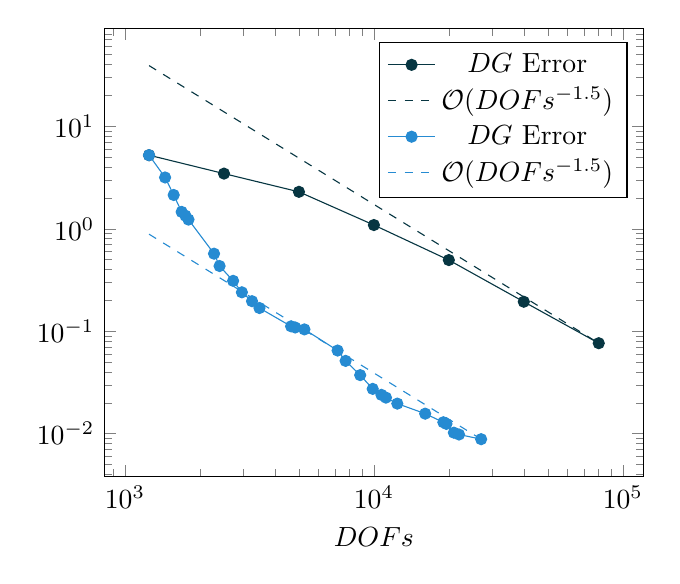
\begin{tikzpicture}
\begin{loglogaxis}[
    xlabel={$DOFs$},
    legend pos=north east,
]

\addplot[solarized-base02, mark=*] coordinates {(1250,5.22824) (2500,3.45593) (5000,2.29411) (10000,1.08811) (20000,0.495229) (40000,0.194102) (80000,0.0764724)};
\addlegendentry{$DG$ Error}

\addplot[solarized-base02, dashed] coordinates {(1250,39.1538688) (80000,0.0764724)};
\addlegendentry{$\mathcal{O}(DOFs^{-1.5})$}

\addplot[\accentcolor, mark=*] coordinates {(1250,5.22824) (1450,3.16847) (1570,2.13764) (1690,1.46207) (1750,1.34315) (1800,1.22937) (2280,0.571535) (2400,0.433165) (2720,0.310514) (2950,0.239953) (3240,0.196515) (3470,0.168581) (4650,0.111757) (4830,0.108861) (5260,0.104274) (7150,0.0648557) (7700,0.0513934) (8810,0.0373304) (9890,0.0273954) (10720,0.0239574) (11180,0.0225082) (12420,0.0196702) (16070,0.0156938) (19010,0.0129343) (19560,0.0124709) (20950,0.0102387) (21970,0.00982763) (26960,0.00884522)};
\addlegendentry{$DG$ Error}

\addplot[\accentcolor, dashed] coordinates {(1250,0.8859790477668384) (26960,0.00884522)};
\addlegendentry{$\mathcal{O}(DOFs^{-1.5})$}

\end{loglogaxis}
\end{tikzpicture}
	\end{subfigure}
    \caption{$DG$ errors vs $DOFs$ comparison between adaptively refined meshes and a sequence of uniform meshes over a square domain. $k = 2$ (left) and $k = 3$ (right).}
\end{figure}

\begin{figure}[!ht]
	\begin{subfigure}[b]{0.45\textwidth}
		% Errors v DOFs template for TikZ.

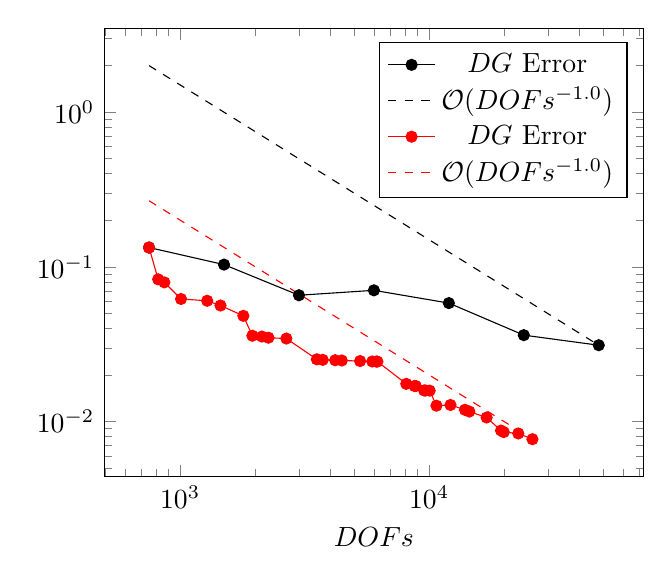
\begin{tikzpicture}
\begin{loglogaxis}[
    xlabel={$DOFs$},
    legend pos=north east,
]

\addplot[black, mark=*] coordinates {(750,0.13327) (1500,0.103364) (3000,0.0655286) (6000,0.0705169) (12000,0.0583046) (24000,0.0362069) (48000,0.0311668)};
\addlegendentry{$DG$ Error}

\addplot[black, dashed] coordinates {(750,1.9946752) (48000,0.0311668)};
\addlegendentry{$\mathcal{O}(DOFs^{-1.0})$}

\addplot[red, mark=*] coordinates {(750,0.13327) (816,0.0830244) (864,0.0793426) (1008,0.0619878) (1284,0.0603523) (1452,0.0562495) (1794,0.0482533) (1950,0.0358904) (2130,0.0354704) (2262,0.0348557) (2670,0.0344147) (3540,0.0252647) (3738,0.0250711) (4194,0.0249254) (4458,0.0248335) (5280,0.0246302) (5910,0.0244758) (6132,0.0244387) (6198,0.0244288) (8094,0.0175423) (8742,0.0169922) (8838,0.0169865) (9546,0.015904) (9660,0.015896) (10050,0.015861) (10698,0.0126811) (12180,0.0128159) (13926,0.0119234) (14502,0.0116229) (17016,0.0106359) (19446,0.00875964) (19938,0.00856267) (22806,0.00838982) (26004,0.00770473)};
\addlegendentry{$DG$ Error}

\addplot[red, dashed] coordinates {(750,0.26713839856000005) (26004,0.00770473)};
\addlegendentry{$\mathcal{O}(DOFs^{-1.0})$}

\end{loglogaxis}
\end{tikzpicture}
	\end{subfigure}
	\hfill
	\begin{subfigure}[b]{0.45\textwidth}
		% Errors v DOFs template for TikZ.

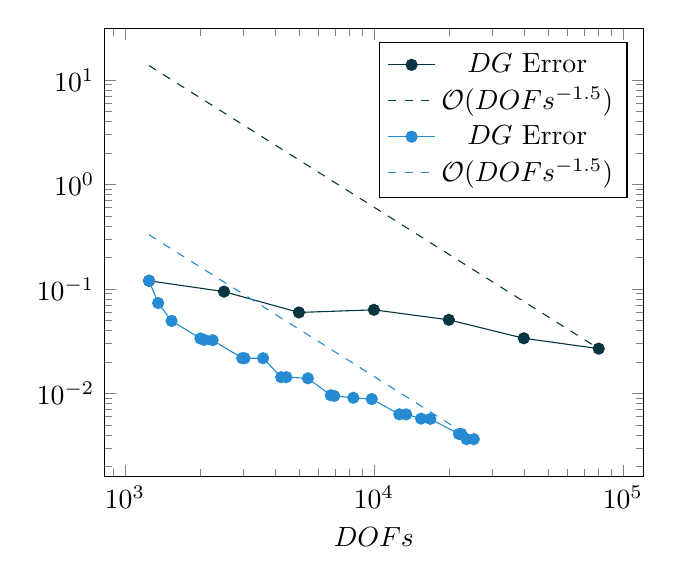
\begin{tikzpicture}
\begin{loglogaxis}[
    xlabel={$DOFs$},
    legend pos=north east,
]

\addplot[solarized-base02, mark=*] coordinates {(1250,0.119546) (2500,0.0940843) (5000,0.0594572) (10000,0.0630071) (20000,0.050544) (40000,0.0336455) (80000,0.0267768)};
\addlegendentry{$DG$ Error}

\addplot[solarized-base02, dashed] coordinates {(1250,13.7097216) (80000,0.0267768)};
\addlegendentry{$\mathcal{O}(DOFs^{-1.5})$}

\addplot[\accentcolor, mark=*] coordinates {(1250,0.119546) (1360,0.0730976) (1540,0.0493759) (2010,0.0335623) (2080,0.0325106) (2250,0.0322421) (2960,0.0217044) (3020,0.0216543) (3590,0.0216774) (4240,0.0142896) (4450,0.0142875) (5430,0.0139307) (6710,0.009591) (6930,0.0094454) (8270,0.00907011) (9800,0.00881814) (12650,0.00629972) (13480,0.00629107) (15470,0.00572756) (16850,0.00569782) (21960,0.00407968) (22460,0.00407912) (23570,0.00364227) (25190,0.00363907)};
\addlegendentry{$DG$ Error}

\addplot[\accentcolor, dashed] coordinates {(1250,0.3292059237674489) (25190,0.00363907)};
\addlegendentry{$\mathcal{O}(DOFs^{-1.5})$}

\end{loglogaxis}
\end{tikzpicture}
	\end{subfigure}
    \caption{$DG$ errors vs $DOFs$ comparison between adaptively refined meshes and a sequence of uniform meshes over an L-shaped domain. $k = 2$ (left) and $k = 3$ (right).}
\end{figure}

\newpage

Due to the nature of the pathological solutions, it may be worth considering adaptive refinement based on local $\HO$ errors rather than $\LT$ errors. The following plots show improved results, particularly for the L-shaped domain.

\begin{figure}[!ht]
	\begin{subfigure}[b]{0.45\textwidth}
		% Errors v DOFs template for TikZ.

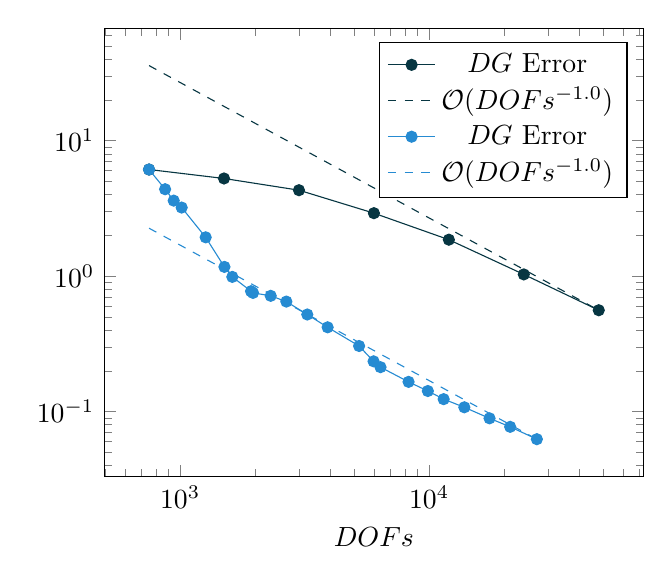
\begin{tikzpicture}
\begin{loglogaxis}[
    xlabel={$DOFs$},
    legend pos=north east,
]

\addplot[solarized-base02, mark=*] coordinates {(750,6.12566) (1500,5.25995) (3000,4.30988) (6000,2.91652) (12000,1.85839) (24000,1.02974) (48000,0.5601)};
\addlegendentry{$DG$ Error}

\addplot[solarized-base02, dashed] coordinates {(750,35.8464) (48000,0.5601)};
\addlegendentry{$\mathcal{O}(DOFs^{-1.0})$}

\addplot[\accentcolor, mark=*] coordinates {(750,6.12566) (870,4.38193) (942,3.60957) (1014,3.20899) (1266,1.93506) (1506,1.16987) (1620,0.987314) (1926,0.773812) (1962,0.752143) (2310,0.715501) (2670,0.648814) (3240,0.520831) (3912,0.419024) (5232,0.304942) (5982,0.234997) (6378,0.212735) (8268,0.165754) (9882,0.141861) (11436,0.123541) (13848,0.107573) (17484,0.0891911) (21156,0.0771805) (27078,0.0625627)};
\addlegendentry{$DG$ Error}

\addplot[\accentcolor, dashed] coordinates {(750,2.2587637207999998) (27078,0.0625627)};
\addlegendentry{$\mathcal{O}(DOFs^{-1.0})$}

\end{loglogaxis}
\end{tikzpicture}
	\end{subfigure}
	\hfill
	\begin{subfigure}[b]{0.45\textwidth}
		% Errors v DOFs template for TikZ.

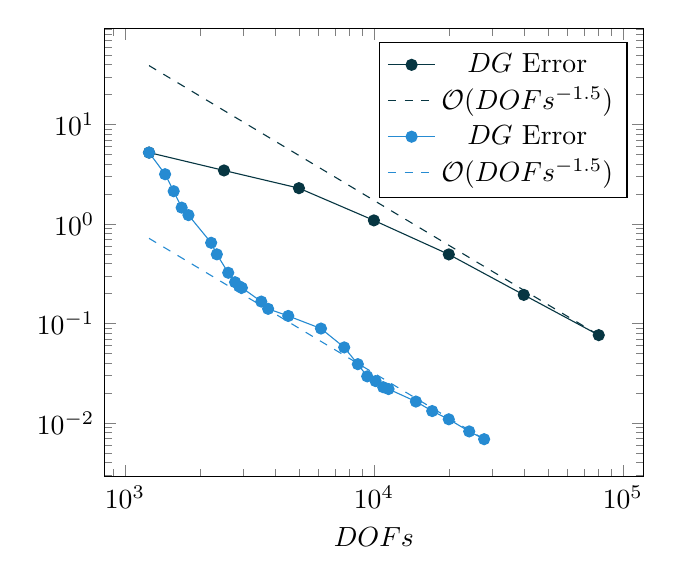
\begin{tikzpicture}
\begin{loglogaxis}[
    xlabel={$DOFs$},
    legend pos=north east,
]

\addplot[solarized-base02, mark=*] coordinates {(1250,5.22824) (2500,3.45593) (5000,2.29411) (10000,1.08811) (20000,0.495229) (40000,0.194102) (80000,0.0764724)};
\addlegendentry{$DG$ Error}

\addplot[solarized-base02, dashed] coordinates {(1250,39.1538688) (80000,0.0764724)};
\addlegendentry{$\mathcal{O}(DOFs^{-1.5})$}

\addplot[\accentcolor, mark=*] coordinates {(1250,5.22824) (1450,3.16847) (1570,2.13764) (1690,1.46207) (1800,1.22937) (2220,0.648223) (2340,0.495982) (2600,0.323852) (2770,0.260152) (2880,0.236183) (2950,0.22874) (3530,0.166199) (3760,0.140521) (4530,0.119187) (6130,0.089056) (7600,0.0575574) (8620,0.0390489) (9400,0.0294453) (10160,0.0263927) (10900,0.0229053) (11450,0.0219544) (14750,0.0164373) (17150,0.0131901) (19990,0.0109056) (24140,0.00823295) (27720,0.00688026)};
\addlegendentry{$DG$ Error}

\addplot[\accentcolor, dashed] coordinates {(1250,0.7185047930727512) (27720,0.00688026)};
\addlegendentry{$\mathcal{O}(DOFs^{-1.5})$}

\end{loglogaxis}
\end{tikzpicture}
	\end{subfigure}
    \caption{$DG$ errors vs $DOFs$ comparison between adaptively refined meshes and a sequence of uniform meshes over a square domain. $k = 2$ (left) and $k = 3$ (right).}
\end{figure}

\begin{figure}[!ht]
	\begin{subfigure}[b]{0.45\textwidth}
		% Errors v DOFs template for TikZ.

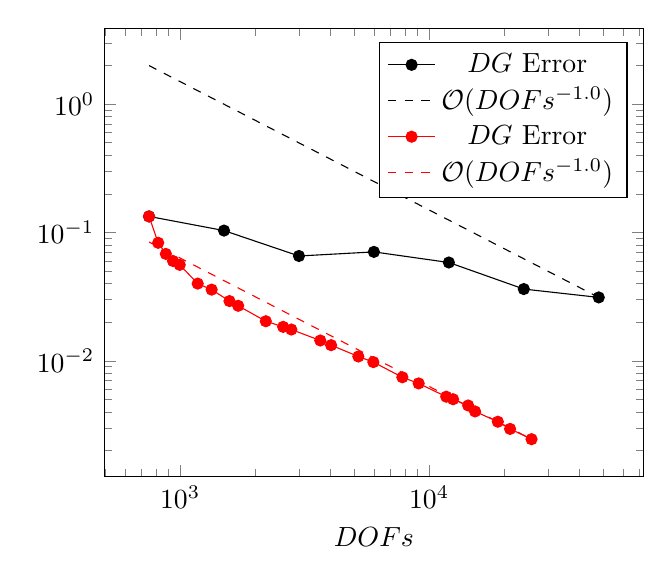
\begin{tikzpicture}
\begin{loglogaxis}[
    xlabel={$DOFs$},
    legend pos=north east,
]

\addplot[black, mark=*] coordinates {(750,0.13327) (1500,0.103364) (3000,0.0655286) (6000,0.0705169) (12000,0.0583046) (24000,0.0362069) (48000,0.0311668)};
\addlegendentry{$DG$ Error}

\addplot[black, dashed] coordinates {(750,1.9946752) (48000,0.0311668)};
\addlegendentry{$\mathcal{O}(DOFs^{-1.0})$}

\addplot[red, mark=*] coordinates {(750,0.13327) (816,0.0830244) (876,0.0680097) (936,0.0598727) (996,0.0559014) (1176,0.039932) (1338,0.0358411) (1578,0.0291867) (1710,0.0268234) (2208,0.0203268) (2592,0.0183746) (2796,0.0175187) (3654,0.0143896) (4038,0.0132366) (5196,0.0107976) (5970,0.00976556) (7806,0.00743953) (9078,0.00666211) (11712,0.00525048) (12480,0.00501671) (14346,0.00448473) (15294,0.00402922) (18876,0.00335053) (21138,0.00294547) (25782,0.00244963)};
\addlegendentry{$DG$ Error}

\addplot[red, dashed] coordinates {(750,0.08420848087999999) (25782,0.00244963)};
\addlegendentry{$\mathcal{O}(DOFs^{-1.0})$}

\end{loglogaxis}
\end{tikzpicture}
	\end{subfigure}
	\hfill
	\begin{subfigure}[b]{0.45\textwidth}
		% Errors v DOFs template for TikZ.

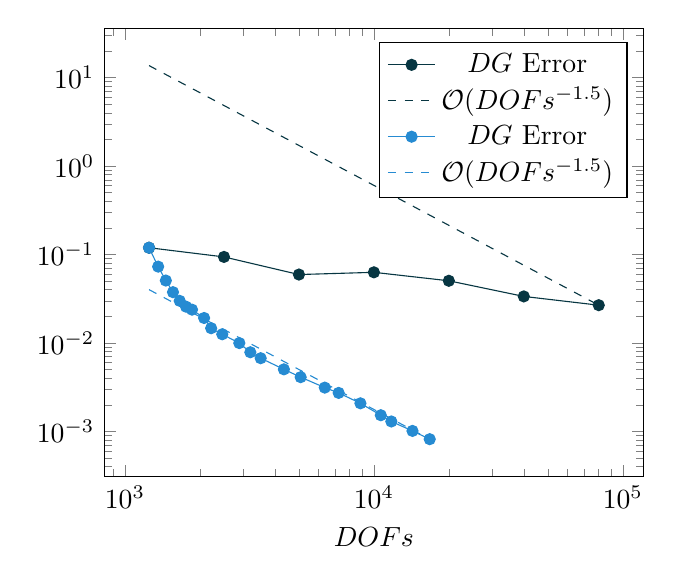
\begin{tikzpicture}
\begin{loglogaxis}[
    xlabel={$DOFs$},
    legend pos=north east,
]

\addplot[solarized-base02, mark=*] coordinates {(1250,0.119546) (2500,0.0940843) (5000,0.0594572) (10000,0.0630071) (20000,0.050544) (40000,0.0336455) (80000,0.0267768)};
\addlegendentry{$DG$ Error}

\addplot[solarized-base02, dashed] coordinates {(1250,13.7097216) (80000,0.0267768)};
\addlegendentry{$\mathcal{O}(DOFs^{-1.5})$}

\addplot[\accentcolor, mark=*] coordinates {(1250,0.119546) (1360,0.0730976) (1460,0.0508708) (1560,0.0375773) (1660,0.0299764) (1760,0.0257653) (1860,0.0238484) (2080,0.0191889) (2220,0.0147015) (2460,0.0125616) (2880,0.00998454) (3190,0.00786125) (3510,0.00673439) (4350,0.0050375) (5080,0.00411082) (6350,0.00313077) (7220,0.00272903) (8830,0.00208062) (10660,0.0015255) (11750,0.00129659) (14290,0.00101426) (16760,0.000817683)};
\addlegendentry{$DG$ Error}

\addplot[\accentcolor, dashed] coordinates {(1250,0.0401449545527477) (16760,0.000817683)};
\addlegendentry{$\mathcal{O}(DOFs^{-1.5})$}

\end{loglogaxis}
\end{tikzpicture} % Incomplete.
	\end{subfigure}
    \caption{$DG$ errors vs $DOFs$ comparison between adaptively refined meshes and a sequence of uniform meshes over an L-shaped domain. $k = 2$ (left) and $k = 3$ (right).}
\end{figure}

\newpage
\subsubsection{Meshes}

Due to localized errors, the meshes are refined in areas where the error is greatest, thereby minimizing the number of degrees of freedom in regions where the solution is already well-approximated.

\begin{figure}[!ht]
	\centering
	\includegraphics[width=5.5cm]{meshes/adaptive/square_h_5.pdf}
	\includegraphics[width=5.5cm]{meshes/adaptive/square_h_10.pdf}
	\includegraphics[width=5.5cm]{meshes/adaptive/square_h_20.pdf}
	\caption{Square mesh after 5, 10 and 20 refinements, $N_0 = 125$.}
\end{figure}

\begin{figure}[!ht]
	\centering
	\includegraphics[width=5.5cm]{meshes/adaptive/lshape_h_5.pdf}
	\includegraphics[width=5.5cm]{meshes/adaptive/lshape_h_10.pdf}
	\includegraphics[width=5.5cm]{meshes/adaptive/lshape_h_20.pdf}
	\caption{L-shaped mesh after 5, 10 and 20 refinements, $N_0 = 125$.}
\end{figure}

\newpage

Meshes refined based on local $\HO$ errors exhibit more concentrated refinement, demonstrating once again the superior approach provided by $\HO$ errors for these particular solutions.

\begin{figure}[!ht]
	\centering
	\includegraphics[width=5.5cm]{meshes/adaptive/square_gh_5.pdf}
	\includegraphics[width=5.5cm]{meshes/adaptive/square_gh_10.pdf}
	\includegraphics[width=5.5cm]{meshes/adaptive/square_gh_20.pdf}
	\caption{Square mesh after 5, 10 and 20 refinements, $N_0 = 125$.}
\end{figure}

\begin{figure}[!ht]
	\centering
	\includegraphics[width=5.5cm]{meshes/adaptive/lshape_gh_5.pdf}
	\includegraphics[width=5.5cm]{meshes/adaptive/lshape_gh_10.pdf}
	\includegraphics[width=5.5cm]{meshes/adaptive/lshape_gh_20.pdf}
	\caption{L-shaped mesh after 5, 10 and 20 refinements, $N_0 = 125$.}
\end{figure}

\newpage
\subsection{A posteriori error estimates}

The second step to implement \textit{h-adaptivity} is to define an \textit{a posteriori} error estimator, enabling the identification of elements that need refinement without requiring any information about the exact solution.

\cite{Cangiani2023} One possible approach considers the following upper bound on the error:

\begin{gather}
	\lVert u - u^k_h \rVert_{\LT(\Omega)} \leq C_{ub} \sum_{K \in \Tau_h} (R_K^2 + O_K^2),
\end{gather}

where:

\begin{gather}
	R_K^2 = R_{K, E}^2 + R_{K, N}^2 + R_{K, J}^2 + R_{K, T}^2
\end{gather}

is the local estimator and:

\begin{gather}
	O_K^2 = O_{K, E}^2 + O_{K, J}^2 + O_{K, T}^2
\end{gather}

is the local data oscillation, with each term given by:

\begin{align}
	R_{K, E} &= \lVert h (\bar{f} + \Delta u^k_h) \rVert_{\LT(K)}, \\
	R_{K, N} &= \lVert h^{1/2} \llbracket \grad u^k_h \cdot \Vector{n} \rrbracket \rVert_{\LT(\partial K)}, \\
	R^2_{K, J} &= \lVert \sigma^{1/2} \llbracket u^k_h \rrbracket \rVert^2_{\LT(\partial K \cap \Gamma_{i})} + \lVert \sigma^{1/2} (u^k_h - \bar{g}) \rVert^2_{\LT(\partial K \cap \partial \Omega)}, \\
	R^2_{K, T} &= \lVert h^{1/2} \llbracket \grad u^k_h \cdot \Vector{e} \rrbracket \rVert^2_{\LT(\partial K \cap \Gamma_{i})} + \lVert \sigma^{1/2} \grad (u^k_h - \bar{g}) \cdot \Vector{e} \rVert^2_{\LT(\partial K \cap \partial \Omega)}, \\
	O_{K, E} &= \lVert h (f - \bar{f}) \rVert_{\LT(K)}, \\
	O_{K, J} &= \lVert \sigma^{1/2} (g - \bar{g}) \rVert_{\LT(\partial K \cap \partial \Omega)}, \\
	O_{K, T} &= \lVert h^{1/2} \grad (g - \bar{g}) \cdot \Vector{e} \rVert_{\LT(\partial K \cap \partial \Omega)}.
\end{align}

Here, $h$ represents the element size, $\sigma$ denotes the penalty coefficient for a given edge, and $\Vector{e}$ represents the unit vector along a given edge for tangent gradients.

\newpage
\subsubsection{Errors}

These error trends demonstrate that the \textit{a posteriori} error estimates (blue) behave similarly to the \textit{a priori} estimates (black). Additionally, in the case of the L-shaped domain, they exhibit improved behavior due to more concentrated refinement in the region of greatest interest. This is due to the significant local data oscillation caused by the singularity of $\grad u$ at the origin for this particular pathological solution.

\begin{figure}[!ht]
	\begin{subfigure}[b]{0.45\textwidth}
		% Errors v DOFs template for TikZ.

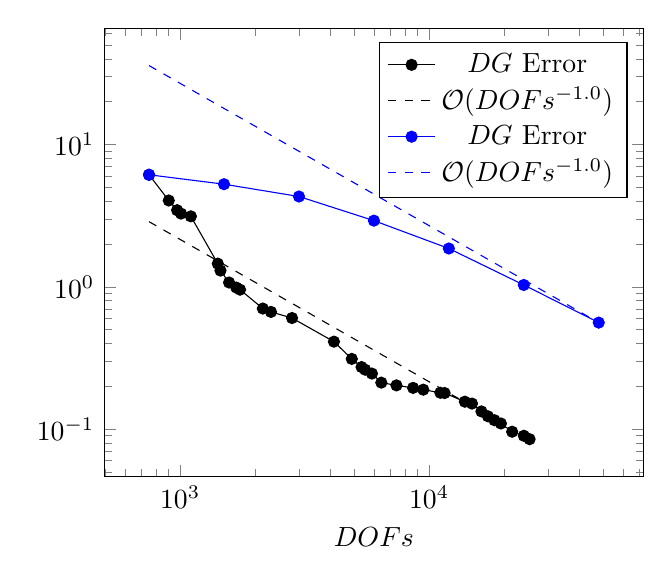
\begin{tikzpicture}
\begin{loglogaxis}[
    xlabel={$DOFs$},
    legend pos=north east,
]

\addplot[black, mark=*] coordinates {(750,6.12566) (900,4.03955) (972,3.45362) (1008,3.26799) (1104,3.12636) (1416,1.45431) (1452,1.30003) (1572,1.0716) (1680,0.987916) (1740,0.954643) (2148,0.70325) (2316,0.666102) (2814,0.603387) (4146,0.411693) (4890,0.311397) (5352,0.272847) (5532,0.261592) (5892,0.245583) (6426,0.212127) (7392,0.202913) (8622,0.194848) (9474,0.189286) (11094,0.180045) (11538,0.179227) (13914,0.155865) (14862,0.151127) (16218,0.133144) (17226,0.123047) (18294,0.11549) (19422,0.109519) (21546,0.0958461) (24006,0.0897779) (25320,0.0849597)};
\addlegendentry{$DG$ Error}

\addplot[black, dashed] coordinates {(750,2.868239472) (25320,0.0849597)};
\addlegendentry{$\mathcal{O}(DOFs^{-1.0})$}

\addplot[blue, mark=*] coordinates {(750,6.12566) (1500,5.25995) (3000,4.30988) (6000,2.91652) (12000,1.85839) (24000,1.02974) (48000,0.5601)};
\addlegendentry{$DG$ Error}

\addplot[blue, dashed] coordinates {(750,35.8464) (48000,0.5601)};
\addlegendentry{$\mathcal{O}(DOFs^{-1.0})$}

\end{loglogaxis}
\end{tikzpicture}
	\end{subfigure}
	\hfill
	\begin{subfigure}[b]{0.45\textwidth}
		% Errors v DOFs template for TikZ.

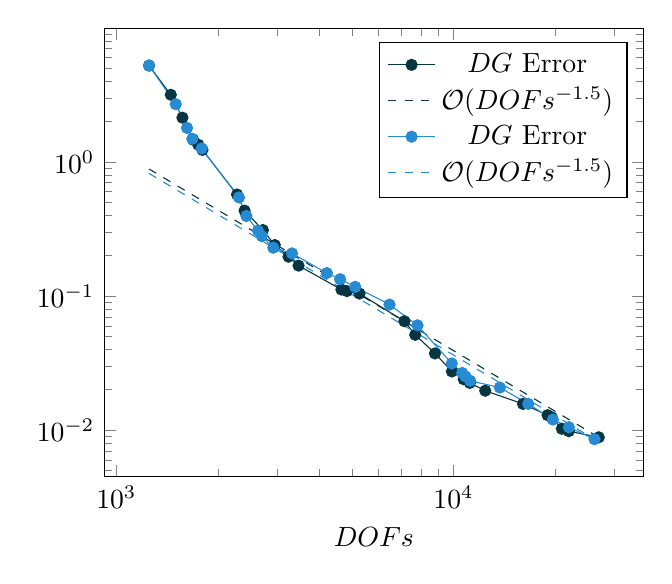
\begin{tikzpicture}
\begin{loglogaxis}[
    xlabel={$DOFs$},
    legend pos=north east,
]

\addplot[solarized-base02, mark=*] coordinates {(1250,5.22824) (1450,3.16847) (1570,2.13764) (1690,1.46207) (1750,1.34315) (1800,1.22937) (2280,0.571535) (2400,0.433165) (2720,0.310514) (2950,0.239953) (3240,0.196515) (3470,0.168581) (4650,0.111757) (4830,0.108861) (5260,0.104274) (7150,0.0648557) (7700,0.0513934) (8810,0.0373304) (9890,0.0273954) (10720,0.0239574) (11180,0.0225082) (12420,0.0196702) (16070,0.0156938) (19010,0.0129343) (19560,0.0124709) (20950,0.0102387) (21970,0.00982763) (26960,0.00884522)};
\addlegendentry{$DG$ Error}

\addplot[solarized-base02, dashed] coordinates {(1250,0.8859790477668384) (26960,0.00884522)};
\addlegendentry{$\mathcal{O}(DOFs^{-1.5})$}

\addplot[\accentcolor, mark=*] coordinates {(1250,5.22824) (1500,2.69514) (1620,1.7934) (1680,1.48702) (1790,1.25894) (2310,0.543447) (2430,0.395368) (2630,0.307434) (2700,0.279644) (2920,0.229209) (3320,0.207952) (4210,0.148303) (4610,0.133591) (5110,0.117099) (6460,0.0863494) (7820,0.0604748) (9880,0.0314321) (10610,0.0267064) (10850,0.0251548) (11200,0.0233236) (13720,0.0207803) (16660,0.0156883) (19710,0.0119851) (21980,0.0105234) (26180,0.00856227)};
\addlegendentry{$DG$ Error}

\addplot[\accentcolor, dashed] coordinates {(1250,0.8206885275389775) (26180,0.00856227)};
\addlegendentry{$\mathcal{O}(DOFs^{-1.5})$}

\end{loglogaxis}
\end{tikzpicture}
	\end{subfigure}
    \caption{$DG$ errors vs $DOFs$ comparison between adaptively refined meshes over a square domain. $k = 2$ (left) and $k = 3$ (right).}
\end{figure}

\begin{figure}[!ht]
	\begin{subfigure}[b]{0.45\textwidth}
		% Errors v DOFs template for TikZ.

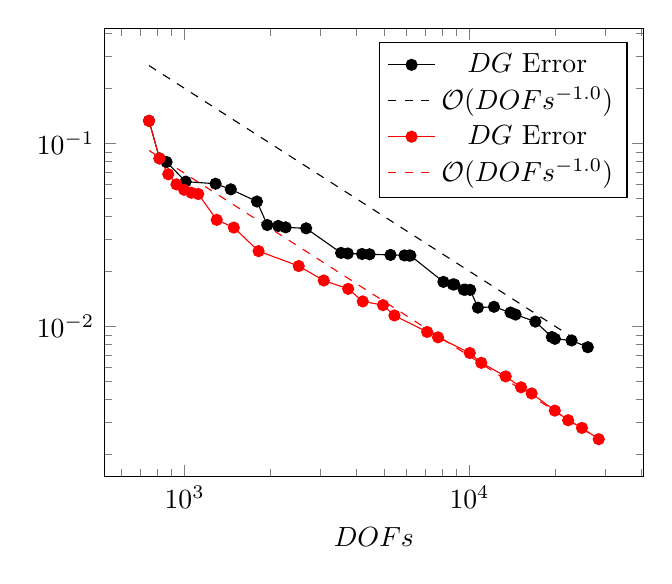
\begin{tikzpicture}
\begin{loglogaxis}[
    xlabel={$DOFs$},
    legend pos=north east,
]

\addplot[black, mark=*] coordinates {(750,0.13327) (816,0.0830244) (864,0.0793426) (1008,0.0619878) (1284,0.0603523) (1452,0.0562495) (1794,0.0482533) (1950,0.0358904) (2130,0.0354704) (2262,0.0348557) (2670,0.0344147) (3540,0.0252647) (3738,0.0250711) (4194,0.0249254) (4458,0.0248335) (5280,0.0246302) (5910,0.0244758) (6132,0.0244387) (6198,0.0244288) (8094,0.0175423) (8742,0.0169922) (8838,0.0169865) (9546,0.015904) (9660,0.015896) (10050,0.015861) (10698,0.0126811) (12180,0.0128159) (13926,0.0119234) (14502,0.0116229) (17016,0.0106359) (19446,0.00875964) (19938,0.00856267) (22806,0.00838982) (26004,0.00770473)};
\addlegendentry{$DG$ Error}

\addplot[black, dashed] coordinates {(750,0.26713839856000005) (26004,0.00770473)};
\addlegendentry{$\mathcal{O}(DOFs^{-1.0})$}

\addplot[red, mark=*] coordinates {(750,0.13327) (816,0.0830244) (876,0.0680097) (936,0.0598727) (996,0.0559014) (1056,0.0538816) (1116,0.0530303) (1296,0.0382955) (1488,0.0347494) (1818,0.0258365) (2514,0.021412) (3078,0.0178477) (3750,0.0160642) (4218,0.0137184) (4968,0.0130898) (5448,0.0114913) (7098,0.0093373) (7752,0.00872489) (10020,0.007165) (10998,0.00633046) (13392,0.00533555) (15168,0.00465232) (16518,0.00430527) (19920,0.00346828) (22188,0.00307256) (24804,0.00278921) (28410,0.00242059)};
\addlegendentry{$DG$ Error}

\addplot[red, dashed] coordinates {(750,0.0916919492) (28410,0.00242059)};
\addlegendentry{$\mathcal{O}(DOFs^{-1.0})$}

\end{loglogaxis}
\end{tikzpicture}
	\end{subfigure}
	\hfill
	\begin{subfigure}[b]{0.45\textwidth}
		% Errors v DOFs template for TikZ.

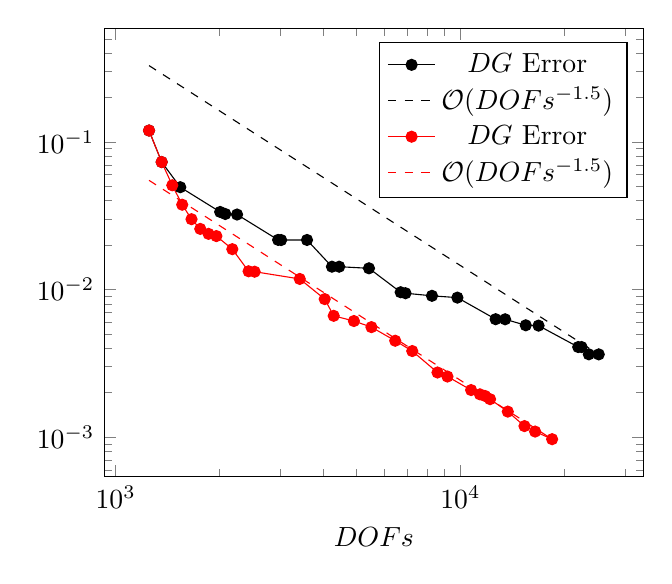
\begin{tikzpicture}
\begin{loglogaxis}[
    xlabel={$DOFs$},
    legend pos=north east,
]

\addplot[black, mark=*] coordinates {(1250,0.119546) (1360,0.0730976) (1540,0.0493759) (2010,0.0335623) (2080,0.0325106) (2250,0.0322421) (2960,0.0217044) (3020,0.0216543) (3590,0.0216774) (4240,0.0142896) (4450,0.0142875) (5430,0.0139307) (6710,0.009591) (6930,0.0094454) (8270,0.00907011) (9800,0.00881814) (12650,0.00629972) (13480,0.00629107) (15470,0.00572756) (16850,0.00569782) (21960,0.00407968) (22460,0.00407912) (23570,0.00364227) (25190,0.00363907)};
\addlegendentry{$DG$ Error}

\addplot[black, dashed] coordinates {(1250,0.3292059237674489) (25190,0.00363907)};
\addlegendentry{$\mathcal{O}(DOFs^{-1.5})$}

\addplot[red, mark=*] coordinates {(1250,0.119546) (1360,0.0730976) (1460,0.0508708) (1560,0.0375773) (1660,0.0299764) (1760,0.0257653) (1860,0.0238484) (1960,0.0230301) (2180,0.0187842) (2430,0.0133021) (2530,0.0132102) (3420,0.0118042) (4040,0.00861783) (4290,0.00663868) (4910,0.00612195) (5520,0.00556495) (6470,0.00450029) (7250,0.00383231) (8580,0.00274332) (9170,0.00257528) (10740,0.00208511) (11390,0.0019513) (11790,0.00190163) (12190,0.0018094) (13720,0.00149002) (15340,0.00118862) (16470,0.00109125) (18450,0.000969034)};
\addlegendentry{$DG$ Error}

\addplot[red, dashed] coordinates {(1250,0.054950108137377836) (18450,0.000969034)};
\addlegendentry{$\mathcal{O}(DOFs^{-1.5})$}

\end{loglogaxis}
\end{tikzpicture} % Incomplete.
	\end{subfigure}
    \caption{$DG$ errors vs $DOFs$ comparison between adaptively refined meshes over an L-shaped domain. $k = 2$ (left) and $k = 3$ (right).}
\end{figure}

\newpage

A better comparison can be made with respect to the $\HO$ refinement, for which the \textit{a posteriori} estimates exhibit the same behavior.

\begin{figure}[!ht]
	\begin{subfigure}[b]{0.45\textwidth}
		% Errors v DOFs template for TikZ.

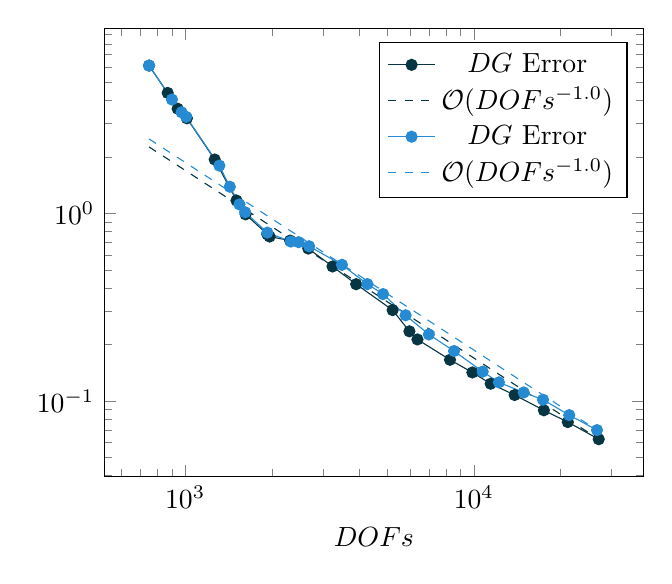
\begin{tikzpicture}
\begin{loglogaxis}[
    xlabel={$DOFs$},
    legend pos=north east,
]

\addplot[solarized-base02, mark=*] coordinates {(750,6.12566) (870,4.38193) (942,3.60957) (1014,3.20899) (1266,1.93506) (1506,1.16987) (1620,0.987314) (1926,0.773812) (1962,0.752143) (2310,0.715501) (2670,0.648814) (3240,0.520831) (3912,0.419024) (5232,0.304942) (5982,0.234997) (6378,0.212735) (8268,0.165754) (9882,0.141861) (11436,0.123541) (13848,0.107573) (17484,0.0891911) (21156,0.0771805) (27078,0.0625627)};
\addlegendentry{$DG$ Error}

\addplot[solarized-base02, dashed] coordinates {(750,2.2587637207999998) (27078,0.0625627)};
\addlegendentry{$\mathcal{O}(DOFs^{-1.0})$}

\addplot[\accentcolor, mark=*] coordinates {(750,6.12566) (900,4.03955) (972,3.45362) (1008,3.26799) (1314,1.79461) (1428,1.38556) (1542,1.11532) (1614,1.01291) (1926,0.78948) (2322,0.707091) (2472,0.701825) (2688,0.667295) (3492,0.531519) (4278,0.419556) (4848,0.371234) (5802,0.286217) (6984,0.22631) (8538,0.184473) (10728,0.143353) (12216,0.125698) (14886,0.111004) (17364,0.101579) (21396,0.0840658) (26706,0.0699521)};
\addlegendentry{$DG$ Error}

\addplot[\accentcolor, dashed] coordinates {(750,2.4908543767999998) (26706,0.0699521)};
\addlegendentry{$\mathcal{O}(DOFs^{-1.0})$}

\end{loglogaxis}
\end{tikzpicture}
	\end{subfigure}
	\hfill
	\begin{subfigure}[b]{0.45\textwidth}
		% Errors v DOFs template for TikZ.

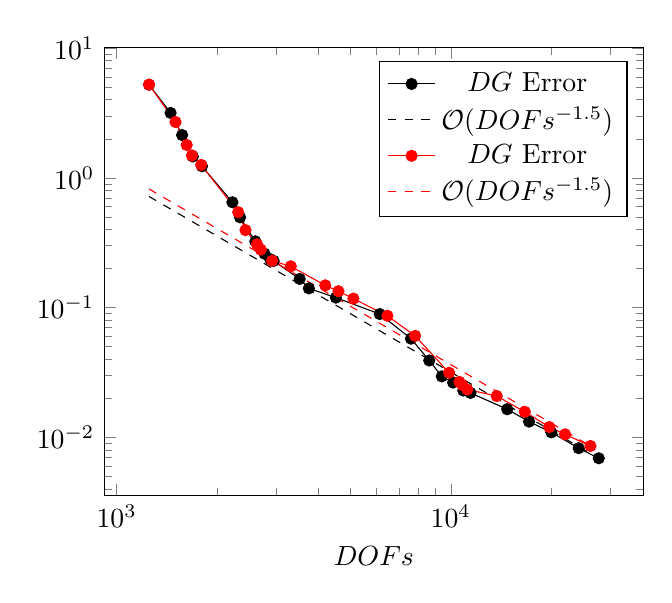
\begin{tikzpicture}
\begin{loglogaxis}[
    xlabel={$DOFs$},
    legend pos=north east,
]

\addplot[black, mark=*] coordinates {(1250,5.22824) (1450,3.16847) (1570,2.13764) (1690,1.46207) (1800,1.22937) (2220,0.648223) (2340,0.495982) (2600,0.323852) (2770,0.260152) (2880,0.236183) (2950,0.22874) (3530,0.166199) (3760,0.140521) (4530,0.119187) (6130,0.089056) (7600,0.0575574) (8620,0.0390489) (9400,0.0294453) (10160,0.0263927) (10900,0.0229053) (11450,0.0219544) (14750,0.0164373) (17150,0.0131901) (19990,0.0109056) (24140,0.00823295) (27720,0.00688026)};
\addlegendentry{$DG$ Error}

\addplot[black, dashed] coordinates {(1250,0.7185047930727512) (27720,0.00688026)};
\addlegendentry{$\mathcal{O}(DOFs^{-1.5})$}

\addplot[red, mark=*] coordinates {(1250,5.22824) (1500,2.69514) (1620,1.7934) (1680,1.48702) (1790,1.25894) (2310,0.543447) (2430,0.395368) (2630,0.307434) (2700,0.279644) (2920,0.229209) (3320,0.207952) (4210,0.148303) (4610,0.133591) (5110,0.117099) (6460,0.0863494) (7820,0.0604748) (9880,0.0314321) (10610,0.0267064) (10850,0.0251548) (11200,0.0233236) (13720,0.0207803) (16660,0.0156883) (19710,0.0119851) (21980,0.0105234) (26180,0.00856227)};
\addlegendentry{$DG$ Error}

\addplot[red, dashed] coordinates {(1250,0.8206885275389775) (26180,0.00856227)};
\addlegendentry{$\mathcal{O}(DOFs^{-1.5})$}

\end{loglogaxis}
\end{tikzpicture}
	\end{subfigure}
    \caption{$DG$ errors vs $DOFs$ comparison between adaptively refined meshes over a square domain. $k = 2$ (left) and $k = 3$ (right).}
\end{figure}

\begin{figure}[!ht]
	\begin{subfigure}[b]{0.45\textwidth}
		% Errors v DOFs template for TikZ.

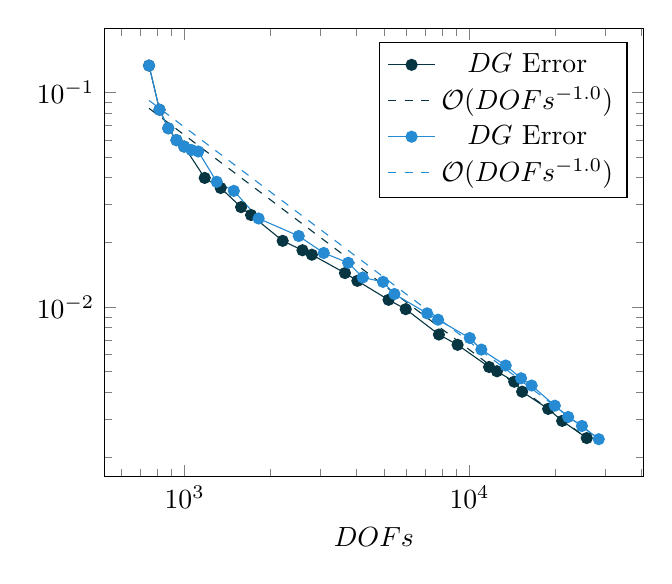
\begin{tikzpicture}
\begin{loglogaxis}[
    xlabel={$DOFs$},
    legend pos=north east,
]

\addplot[solarized-base02, mark=*] coordinates {(750,0.13327) (816,0.0830244) (876,0.0680097) (936,0.0598727) (996,0.0559014) (1176,0.039932) (1338,0.0358411) (1578,0.0291867) (1710,0.0268234) (2208,0.0203268) (2592,0.0183746) (2796,0.0175187) (3654,0.0143896) (4038,0.0132366) (5196,0.0107976) (5970,0.00976556) (7806,0.00743953) (9078,0.00666211) (11712,0.00525048) (12480,0.00501671) (14346,0.00448473) (15294,0.00402922) (18876,0.00335053) (21138,0.00294547) (25782,0.00244963)};
\addlegendentry{$DG$ Error}

\addplot[solarized-base02, dashed] coordinates {(750,0.08420848087999999) (25782,0.00244963)};
\addlegendentry{$\mathcal{O}(DOFs^{-1.0})$}

\addplot[\accentcolor, mark=*] coordinates {(750,0.13327) (816,0.0830244) (876,0.0680097) (936,0.0598727) (996,0.0559014) (1056,0.0538816) (1116,0.0530303) (1296,0.0382955) (1488,0.0347494) (1818,0.0258365) (2514,0.021412) (3078,0.0178477) (3750,0.0160642) (4218,0.0137184) (4968,0.0130898) (5448,0.0114913) (7098,0.0093373) (7752,0.00872489) (10020,0.007165) (10998,0.00633046) (13392,0.00533555) (15168,0.00465232) (16518,0.00430527) (19920,0.00346828) (22188,0.00307256) (24804,0.00278921) (28410,0.00242059)};
\addlegendentry{$DG$ Error}

\addplot[\accentcolor, dashed] coordinates {(750,0.0916919492) (28410,0.00242059)};
\addlegendentry{$\mathcal{O}(DOFs^{-1.0})$}

\end{loglogaxis}
\end{tikzpicture}
	\end{subfigure}
	\hfill
	\begin{subfigure}[b]{0.45\textwidth}
		% Errors v DOFs template for TikZ.

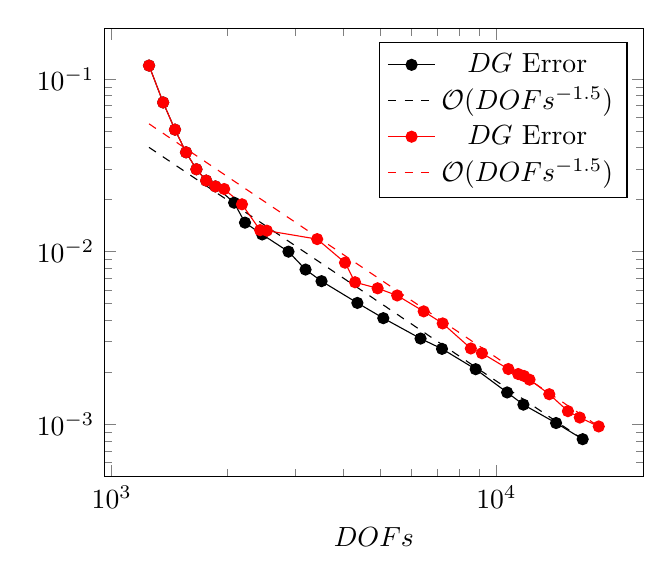
\begin{tikzpicture}
\begin{loglogaxis}[
    xlabel={$DOFs$},
    legend pos=north east,
]

\addplot[black, mark=*] coordinates {(1250,0.119546) (1360,0.0730976) (1460,0.0508708) (1560,0.0375773) (1660,0.0299764) (1760,0.0257653) (1860,0.0238484) (2080,0.0191889) (2220,0.0147015) (2460,0.0125616) (2880,0.00998454) (3190,0.00786125) (3510,0.00673439) (4350,0.0050375) (5080,0.00411082) (6350,0.00313077) (7220,0.00272903) (8830,0.00208062) (10660,0.0015255) (11750,0.00129659) (14290,0.00101426) (16760,0.000817683)};
\addlegendentry{$DG$ Error}

\addplot[black, dashed] coordinates {(1250,0.0401449545527477) (16760,0.000817683)};
\addlegendentry{$\mathcal{O}(DOFs^{-1.5})$}

\addplot[red, mark=*] coordinates {(1250,0.119546) (1360,0.0730976) (1460,0.0508708) (1560,0.0375773) (1660,0.0299764) (1760,0.0257653) (1860,0.0238484) (1960,0.0230301) (2180,0.0187842) (2430,0.0133021) (2530,0.0132102) (3420,0.0118042) (4040,0.00861783) (4290,0.00663868) (4910,0.00612195) (5520,0.00556495) (6470,0.00450029) (7250,0.00383231) (8580,0.00274332) (9170,0.00257528) (10740,0.00208511) (11390,0.0019513) (11790,0.00190163) (12190,0.0018094) (13720,0.00149002) (15340,0.00118862) (16470,0.00109125) (18450,0.000969034)};
\addlegendentry{$DG$ Error}

\addplot[red, dashed] coordinates {(1250,0.054950108137377836) (18450,0.000969034)};
\addlegendentry{$\mathcal{O}(DOFs^{-1.5})$}

\end{loglogaxis}
\end{tikzpicture} % Incomplete.
	\end{subfigure}
    \caption{$DG$ errors vs $DOFs$ comparison between adaptively refined meshes over an L-shaped domain. $k = 2$ (left) and $k = 3$ (right).}
\end{figure}

\newpage
\subsubsection{Meshes}

These meshes exhibit a more concentrated refinement compared to those refined using \textit{a priori} error estimates.

\begin{figure}[!ht]
	\centering
	\includegraphics[width=5.5cm]{meshes/adaptive/square_eh_5.pdf}
	\includegraphics[width=5.5cm]{meshes/adaptive/square_eh_10.pdf}
	\includegraphics[width=5.5cm]{meshes/adaptive/square_eh_20.pdf}
	\caption{Square mesh after 5, 10 and 20 refinements, $N_0 = 125$.}
\end{figure}

\begin{figure}[!ht]
	\centering
	\includegraphics[width=5.5cm]{meshes/adaptive/lshape_eh_5.pdf}
	\includegraphics[width=5.5cm]{meshes/adaptive/lshape_eh_10.pdf}
	\includegraphics[width=5.5cm]{meshes/adaptive/lshape_eh_20.pdf}
	\caption{L-shaped mesh after 5, 10 and 20 refinements, $N_0 = 125$.}
\end{figure}

\newpage
\subsection{A code snippet}

Here's a snippet to illustrate the \textit{h-adaptive} mesh refinement from the user's perspective:

\lstinputlisting[style=cpp, firstline=11]{../snippets/h_refine.cpp}

	\newpage
    \section{Implementing \textit{hp-Adaptivity}}
	

\newpage
\subsection{A code snippet}

Here's a snippet to illustrate the \textit{hp-adaptive} mesh refinement from the user's perspective:

\lstinputlisting[style=cpp, firstline=11]{../snippets/hp_refine.cpp}

	\newpage
    \section{Conclusion}
	This report has provided a comprehensive study of adaptive mesh refinement strategies within the context of the Discontinuous Galerkin (DG) method, focusing on both \textit{h-adaptivity} and \textit{p-adaptivity}.

The evaluation of \textit{h-adaptive} refinement strategies demonstrated their effectiveness in managing complex geometries and solutions with local singularities. This approach effectively reduces local discretization errors by refining the mesh where needed.

In the domain of \textit{p-adaptivity}, the analysis of the decay rates of Legendre coefficients proved to be a reliable method for assessing solution smoothness and guiding polynomial order adjustments. The results confirmed that starting with a higher polynomial order, such as $k = 3$, leads to more accurate decay rate estimates and improved convergence behavior.

A comparison of \textit{h-adaptive} and \textit{hp-adaptive} refinement strategies highlighted their respective advantages. While \textit{h-adaptivity} effectively manages local errors through mesh refinement, \textit{hp-adaptivity} offers additional benefits by adjusting polynomial orders alongside mesh resolution.

Overall, the results of this project underscore the practical benefits of adaptive refinement strategies in DG methods. By utilizing a posteriori error estimators, \textit{h-adaptivity} and \textit{hp-adaptivity} can be effectively implemented to achieve accurate and efficient numerical solutions.

	\newpage
	\addcontentsline{toc}{section}{References}
	\bibliography{bibliography/refs.bib}
	\bibliographystyle{siam}

\end{document}
